\documentclass[12pt]{article}
\usepackage[a4paper, margin=.30in]{geometry}
\usepackage{graphicx ,
            wrapfig,
            xcolor, 
            enumerate,
            amsmath,fontenc,makecell,chemfig, multirow
            }

\newcommand\headerMe[2]{\noindent{}#1\hfill#2}
\renewcommand{\thesection}{\Roman{section}}

%\title{Leçon N 6 : Le mouvement}
\author{Zakaria HAOUZAN}
\date{\today}

\begin{document}
% headers --------------
\headerMe{Matière : Physique-Chimie}{Professeur : Zakaria HAOUZAN}\\
\headerMe{Unité : La chimie autours de nous }{Établissement : Lycée SKHOR qualifiant}\\
\headerMe{Niveau : TCS}{Heure : 3H}\\

% ------Content ________
\begin{center}

    \Large{Leçon $N^{\circ} 2 $: \color{red} Extraction, séparation et identification d'espèces chimiques.}
\end{center}

%\begin{wrapfigure}[10]{r}{0.5\textwidth}
%    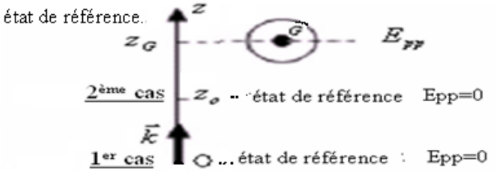
\includegraphics[width=0.5\textwidth]{./img/img00.png}
%\end{wrapfigure}

\section{Situation problème :  }
Dès l’Antiquité, l’homme se servait de substances odorantes pour sa nourriture, embaumer ses morts, se soigner
ou même se parfumer. Plusieurs techniques étaient utilisées :

\begin{enumerate}
	\item \textbf{L’enfleurage :}est utilisé avec des pétales de fleurs
moyennement fragiles (rose, par exemple) qui sont plongées
dans un bain de graisse animale qui est chauffée à plusieurs
reprises. Lorsque les fleurs ont livré toute leur essence, elles
sont enlevées et remplacées par d’autres, et ce, jusqu’à
l’obtention d’une graisse saturée. On obtient, ainsi, une 
pommade  d’enfleurage qui pourra être utilisée comme parfum solide.
L’enfleurage à froid est utilisé avec des pétales de fleurs fragiles (jasmin, par exemple). Le principe est
identique, mais les pétales sont disposés sur une plaque de graisse froide. Cette méthode n’est pratiquement
plus utilisée aujourd’hui car trop coûteuse

\item \textbf{Pressage :} Cette opération consiste à "faire sortir"  un
produit en exerçant une pression. Les Égyptiens écrasaient des
fleurs pour extraire des arômes ou des parfums ; c’est aussi
l’opération effectuée lorsqu’on se prépare l’huile d’olive
\end{enumerate}


\vspace{-1cm}
\section{Techniques d'extraction d'une espèce chimique: }
\subsection{Hydrodistillation: solide-liquide }
\subsubsection{Principe de l'hydrodistillation:}
L'hydrodistillation est une technique permettant d'extraire des espèces chimiques volatiles contenues dans un produit
naturel (plantes , feuilles....) en le faisant bouillir dans l'eau .

La vapeur d'eau entraine avec elle l'espèce chimique
(qui peut être l'huile essentielle de la plante qu'on a chauffé).Le mélange des vapeurs d'eau et d'huile essentielle et ensuite
condensé (rendu liquide) par un réfrigérant pour obtenir un liquide appelé distillat.

Donc l'hydrodistillation est une vaporisation suivie d'une condensation.

\subsubsection{Montage expérimental de l'hydrodistillation:}

\begin{center}
	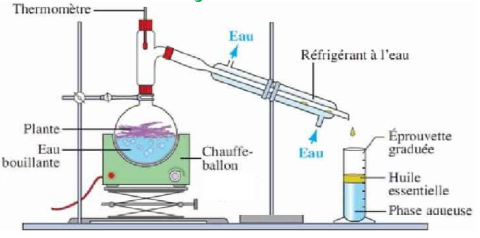
\includegraphics[width=0.5\textwidth]{./img/Extraction_01.png}
\end{center}

\subsubsection{Etape de relargage:}
Le relargage est une technique qui consiste à séparer une substance en solution de son solvant en introduisant une
autre substance plus soluble qui prend sa place.

On ajoute au distillat (espèce chimique +d'eau) obtenu , du chlorure de sodium solide. On agite jusqu'à dissolution complète du sel. 

Cette étape de relargage consiste à rendre l'espèce à extraire moins soluble dans l'eau. Après on
procède par une extraction à l'aide d'un solvant .

\subsection{Extraction par solvant: (ou extraction liquide-liquide) }
\subsubsection{Principe:}
L'extraction par un solvant (ou extraction liquide-liquide) permet d'extraire

une espèce chimique dissoute dans un solvant, à l'aide d'un autre solvant , appelé solvant extracteur .

\subsubsection{Choix du solvant extracteur:}
Généralement le solvant extracteur doit être : volatil ,de faible densité et non miscible avec l'eau.

En plus l'espèce chimique à extraire doit être plus soluble dans le solvant extracteur .Ce qui permet de les séparer en
utilisant une ampoule à décanter.

\subsubsection{Décantation:}

On appelle décantation la séparation de deux liquides non miscibles à
l'aide d'une ampoule à décantation , dans laquelle le mélange se sépare en deux phases non miscibles: Une phase
aqueuse, en général plus dense, se situe dans la partie inférieure et une phase organique ( qui contient l'espèce
chimique à extraire ) de densité plus faible .

\begin{center}
	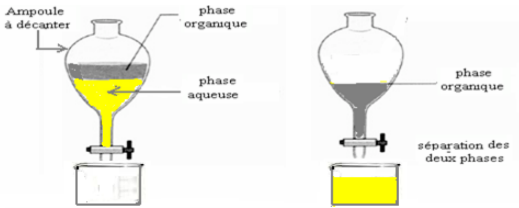
\includegraphics[width=0.5\textwidth]{./img/Extraction_02.png}
\end{center}

\begin{itemize}
	\item L’espèce chimique à extraire est plus soluble dans le solvant extracteur que dans le solvant de départ.
	\item  le solvant extracteur et le solvant de départ sont non miscibles.

	\item Pour extraire une espèce dissoute dans un solvant S1, on utilise un autre solvant S2, non miscible avec S1, dans
lequel l’espèce chimique est nettement plus soluble.
\item  L’extraction par un solvant consiste à dissoudre l’espèce chimique recherchée dans un solvant non miscible
avec l’eau et à séparer les deux phases obtenues.
\item L’extraction par un solvant se réalise dans une ampoule à décanter.
\item Le choix du solvant dépend de l’espèce chimique recherchée.
\item  L’espèce chimique doit être plus soluble dans le solvant que dans l’eau.
\end{itemize}
\subsubsection{Etapes extraction par solvant :}

\begin{center}
	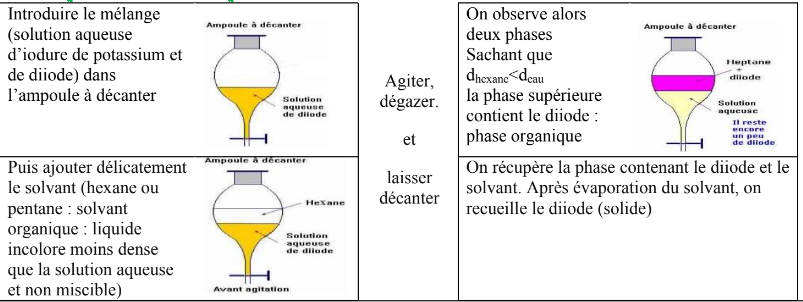
\includegraphics[width=1\textwidth]{./img/Extraction_03.png}
\end{center}

\begin{wrapfigure}[0]{r}{0.3\textwidth}

\vspace{-1cm}
	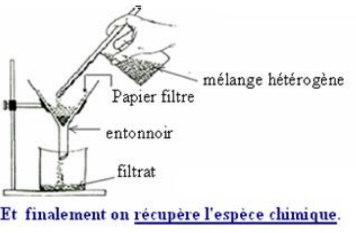
\includegraphics[width=0.3\textwidth]{./img/Extraction_04.png}
\end{wrapfigure}



\section*{Remarque : }
La filtration permet de séparer
les constituants d'un melange qui possède


une phase liquide et une phase solide
au travers un papier filtre.


\section{Techniques de séparation et d'identification des espèces chimiques: }
\subsection{ Chromatographie sur couche mince : }
La chromatographie sur couche mince est une autre méthode de séparation et d'identification des espèces chimiques .

C'est une méthode physique permettant de séparer et d'identifier les constituants d'une solution . Elle se fait
en trois étapes: 

\begin{itemize}

	\item \textbf{1- La première étape :preparation de la plaque: }
		\begin{itemize}
			\item On prend une plaque qui constitue la phase fixe.
			\item On trace à l'aide d'un crayon une ligne appelée ligne de dépôt à environ 1cm de l'extrémité inférieure de la plaque
( et une ligne en haut à environ 6cm appelée front du solvant ) .


\item On pose une goutte de chaque solution à analyser de telle sorte que les points de dépôt soient alignés et espacés.

\item Ensuite on place cette plaque dans un bécher contenant un solvant (l'éluant ,phase mobile). Celui-ci va entrainer
les espèces chimiques à des vitesse différentes.
		\end{itemize}
\end{itemize}
\begin{center}
	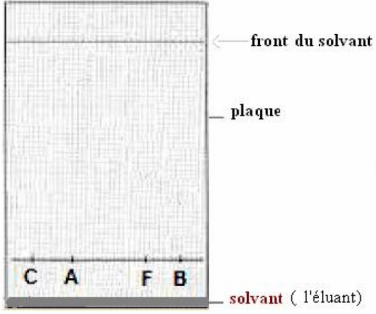
\includegraphics[width=0.3\textwidth]{./img/Exrtaction_05.png}
	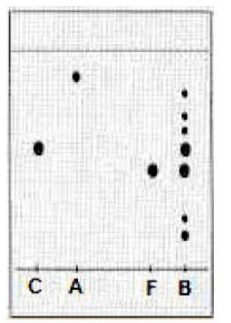
\includegraphics[width=0.2\textwidth]{./img/Extraction_06.png}
\end{center}

On utilise cette méthode pour identifier les constituants d'un mélange en posant à coté d'une goutte par exemple du
mélange B des gouttes d'espèces chimiques C,A et F connues ( références ).

\underline{Attention: }Au début les dépots ne doivent pas être dans l'éluant (car ils seront alors dissous directement dans le
liquide et ils ne monteront pas le long de la plaque).

\begin{itemize}
	\item \textbf{La deuxième étape: analyse du chromatogramme }
		\begin{itemize}
			\item Le chromatogramme est le résultat de la chromatographie
			\item Par absorption et solubilité l’éluant monte lentement à travers la phase stationnaire ainsi que les solutions à
analyser.
\item On fait sortir la plaque lorsque le front de l'éluant atteind sa valeur maximale.
\item On la plonge alors dans un révélateur (solution de permanganate de potassium ou sécher la plaque au sèche-cheveux.
) qui fait apparaître sous forme de tâches les hauteurs atteintes par les différents constituants.

\item Les espèces chimiques sont caractérisées par les hauteurs qu'elles ont atteintes lors de l'élution.

		\end{itemize}
	\item Si l'espèce chimique étudiée donne une seule tache : on dit qu'il s'agit d'un corps pur..
	\item Deux espèces chimiques qui se trouvent sur la même ligne horizontales ont les mêmes propriétés

\end{itemize}

Après analyse de la plaque , on constate que C , A et F donnent une seule tache : ce sont des espèces chimiques
(c'est-à-dire des cops purs).

Et on conclu que le mélange B contient les espèces chimiques C et F. ( mais il ne contient A).

\begin{itemize}

\item \textbf{La troisième étape: (exploitation des résultas)}

\item Le rapport frontal: On caractérise les espèces chimiques par leurs rapports frontal Rf qui ne dépend que de la phase fixe de l'éluant et donné par la relation suivante:
	
\item $$R_f = \frac{h}{H}$$
\item h : hauteur atteinte par l’espèce étudiée
\item H :hauteur atteinte par
l’éluant

\item Les espèces chimiques qui ont le même rapport frontal sont identiques.

\end{itemize}
\begin{center}
	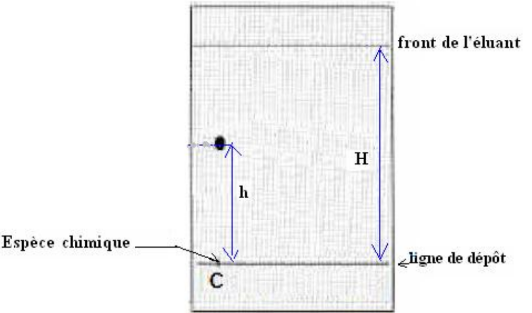
\includegraphics[width=0.6\textwidth]{./img/Extraction_07.png}
\end{center}



\section{Les caractéristiques physiques:}
Toute espèce chimique possède des propriétés physiques dont les valeurs lui sont propres, on les nomme
caractéristiques physiques .

Elles permettent de l'identifier.
Tout corps pur est caractérisé par un ensemble de propriétés physiques qui permettent de le distinguer des autres.

\subsection{Exemples : }
\textbf{La température de fusion : }:C'est la température $\theta_f$ de passage de l'état solide à l'état liquide. 

(Pour un corps pur ce changement d'état se fait à température constante).

La matière qui nous entoure se trouve sous trois états physiques l'état liquide , l'état solide et l'état gazeux. On
appelle changement d'état le passage d'un état physique à autre état

\textbf{La température d'ébullition :}
:C'est la temperature $\theta$éb de passage de l'état liquide à l'état gazeux ,elle se mesure avec un thermomètre pour l'ébullition des liquides.. Tout comme la fusion, l'ébullition est un changement d'état qui se fait à température constante pour un corps pur.

\textbf{La masse volumique:} $$\rho = \frac{m}{V}$$

\textbf{La densité: }$$d = \frac{\rho}{\rho_{eau}}$$
\end{document}

